\section{Design Considerations}
\label{sec:motivation}

\subsection{The Case for Giza}

\begin{figure}[tp]
%\centering
\hspace{-4em}
\begin{subfigure}{.3\textwidth}
  \centering
  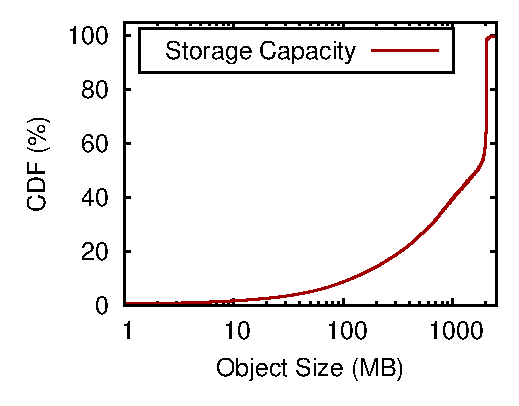
\includegraphics[width=\linewidth]{data/object_size-storage_capacity}
  \caption{}
  \label{fig:object_size-storage_capacity}
\end{subfigure}%
%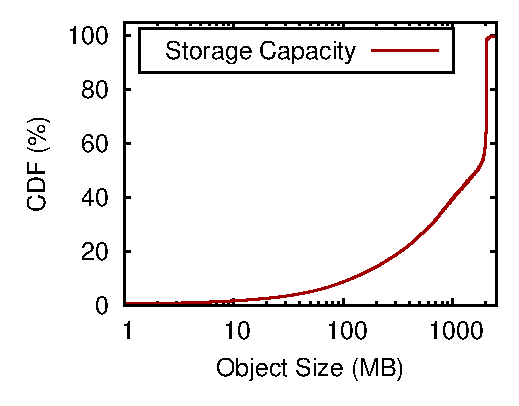
\includegraphics[width=0.5\textwidth]{data/object_size-storage_capacity}
%\hspace{-.5em}
\begin{subfigure}{.3\textwidth}
  \centering
  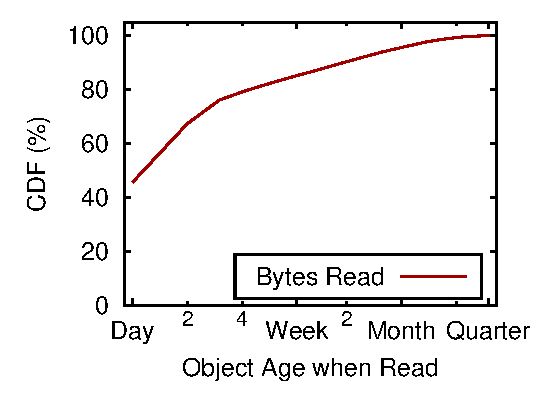
\includegraphics[width=\linewidth]{data/write_read_gap-bytes_read}
  \caption{}
  \label{fig:write_read_gap-bytes_read}
\end{subfigure}%
\caption{Cloud Drive Workload}
\label{fig:case_for_giza}
\end{figure}

\begin{table}[tp]
\centering
\begin{tabular}{|c||c|c|}
\hline \hline
total reads (B) / writes (B) 	& \multicolumn{2}{c|}{2.3$\times$}
\\ \hline \hline
%\multirow{4}{*}{cross-DC reads / writes \newline in Giza}
	& no caching		& 1.15$\times$
\\ \cline{2-3}
cross-DC reads / writes
	& caching (day)		& 0.61$\times$ 
\\ \cline{2-3}
with Giza
	& caching (week)	& 0.18$\times$ 
\\ \cline{2-3}
	& caching (month)	& 0.05$\times$ 
\\ \hline \hline
\end{tabular}
\caption{Giza with Caching in Local DC.}
\label{tab:caching}
\end{table}

%\subsection{Giza: Flexible Cross-DC erasure coding }
%
%Erasure coding across geo-graphically distributed data centers is a most effective approach to reduce storage cost while achieving the fault tolerance goal of being able to survive data center failure. As Facebook's F4 system~\ref{bib:F4} has demonstrated, replacing geo-replication with cross-DC erasure coding can effectively reduce storage overhead from 3.6x to 2.1x, achieving huge savings for Facebook's 65PB of warm storage. While a fixed 2 + 1 solution works very well for Facebook's special workload, the public cloud storage desires much more flexibility. Different customers have different desirable operating points in terms of cost, durability and latency trade-off and are willing to accept different pricing for individual needs. 
%
%Giza provide completes flexibility to the customers. When a storage account is created, the customers may specify how much fault tolerance is desired at the storage account level. In addition, the customers had additional flexibility to specify which data centers are involved, so that they could constraint all the data to be in the  United States per data sovereignty requirement and regulation, or they could choose to disperse the erasure coded data across multiple continents, so that no single country could gain access to the complete data. 


\begin{table*}[tp]
\centering
\begin{tabular}{|l||c||c|c|c|c||c|c|}
\hline
				& Geo-Replication    	& \multicolumn{4}{c||}{Giza (standard durability)}		& \multicolumn{2}{c|}{Giza (enhanced durability)}
\\ \hline \hline
Number of DCs 				& 2										& 3 & 4 & 5 & 6									& 5 & 6
\\ \hline
Erasure coding scheme & replication					& 2 + 1 & 3 + 1 & 4 + 1 & 5 + 1	& 3 + 2 & 4 + 2
\\ \hline \hline
Storage overhead			& 2.6x								& 1.9x & 1.7x & 1.6x & 1.5x			& 2.1x & 1.9x
\\ \hline
Reduction							& -										& 27\% & 35\% & 38\% & 42\%			& 19\% & 27\%
\\ \hline \hline
WAN traffic (put)			& 1x									& 1x & 1x & 1x & 1x 						& 1.33x & 1.25x
\\ \hline
WAN traffic (get)			& 0										& 0.5x & 0.67x & 0.75x & 0.8x		& 0.67x & 0.75x
\\ \hline
DC rebuild 						& 1x									& 2x & 3x & 4x & 5x 						& 3x & 4x
\\ \hline \hline
\end{tabular}
\caption{Trade-off of storage, bandwidth and durability.}
\label{tab:cost_benefit}
\end{table*}


\subsection{Storage, Bandwidth and Durability}

Giza offers the customers the flexibility to specify erasure coding scheme, which results in different operating points in terms of storage overhead, bandwidth cost and durability.

\subsubsection{Storage and Durability}

With standard durability, Giza applies $k+1$ erasure coding, which stores $k+1$ coded fragments in different data centers and tolerates single data center failure. With enhanced durability, Giza applies $k+2$ erasure coding, which stores coded fragments in $k+2$ data centers. This tolerates arbitrary 2 data center failures and achieves much higher durability. 

Table~\ref{tab:cost_benefit} compares the costs and benefits of Giza at various operating points to geo-replication.
To tolerate single data center failure, geo-replication requires a storage overhead of $2\times1.3$ = 2.6 (where single DC storage overhead is a constant at 1.3). With $k+1$ erasure coding, where $k$ ranges from 2 to 5, Giza reduces the storage overhead to between 1.9 and 1.5, a reduction of 27\% to 42\%. Even with enhanced durability tolerating 2 data center failures, Giza again reduces the storage overhead to between 2.1 to 1.9, a reduction of 19\% to 27\%. As summarized Table~\ref{tab:cost_benefit}, compared to geo-replication, Giza achieves comparable durability while significantly reducing storage overhead, or much higher durability while still reducing storage overhead substantially.

Nevertheless, the reduction in storage overhead comes at the additional cost of inflated cross-DC network traffic, which is examined next.

\subsubsection{Constant Cross-DC Traffic for Put}

Let's revisit the example of storing the 4MB data object. In geo-replication, in addition to being stored in a local DC, the object is replicated and stored in a remote DC. The replication incurs 1x of cross-DC traffic. Giza, with $2 + 1$ erasure coding, divides the object  and generates 3 coded fragments ($a$, $b$ and $p$) with 2MB each. It stores 1 fragment in the local DC and replicates 2 fragments to two remote DCs. The replication again incurs 1x cross-DC traffic, the same as geo-replication. In general, with $k+1$ erasure coding, the cross-DC traffic is constant for both geo-replication and cross-DC erasure coding.

The analysis readily extends to $k+2$ erasure coding. As shown in Table~\ref{tab:cost_benefit}, the cross-DC traffic is slightly higher than geo-replication, inevitable to achieve higher durability.

\subsubsection{Inflated Cross-DC Traffic for Get and Rebuild}

In geo-replication, each data center has the full copy of the data object. {\em Get} can access the local DC and incur no cross-DC traffic. In contrast, with $2+1$ erasure coding, Giza can only read half of the object from the local DC. Reading the other half from a remote DC always incurs cross-DC traffic, a $0.5$$\times$ unit for {\em get}. Generalizing the argument, Table~\ref{tab:cost_benefit} shows that the higher $k$ is (in $k+1$ erasure coding), the higher cross-DC traffic {\em get} incurs.

When a data center fails, customer data originally stored at the failed DC needs to be rebuilt at a new DC. Geo-replication simply replicates every data object and thus incurs 1x of cross-DC traffic. In contrast, Giza applies erasure decoding to reconstruct missing fragments, each incurring $k$ times cross-DC traffic for arbitrary $k+m$ erasure coding.

\subsection{Alternative Approach}
\label{sec:alternative}

%\ch{It feels better to move this subsection to a later section dedicated for discussion. We could mention Haibo's work there, or better in the related work section. If we do that, the tile of this section should probably be changed to ``costs and benefits''.}

Giza treats data objects independently. To store a data object, Giza splits the object into multiple data fragments and generates parity fragments. All the coded fragments are dispersed and stored in different data centers. To retrieve the object, Giza reads enough coded fragments from the multiple data centers and reconstructs the data object. Hence, Giza always incurs cross-DC traffic when reading object.

The decision to treat data objects independently is a deliberate choice after careful considerations of alternative approaches. One viable alternative is to first aggregate objects into logical volumes and then erasure code across different volumes. For instance, objects in data center A are aggregated into $vol_A$ and those in data center B into $vol_B$. Volumes are large, say in the order of 100GB. A parity volume $vol_P$ is generated by erasure coding $vol_A$ and $vol_B$, which is stored in yet another data center C.

This approach avoids cross-DC traffic when reading individual objects, as every object is available in its entirety in one of the DCs. However, the challenge of this approach is to handle object deletion. Whenever an object is deleted from $vol_A$ in data center A, it needs to be transmitted to data center C so as to be {\em canceled} from $vol_C$. Hence, object deletion incurs cross-DC traffic. In addition, deleting objects from the logical volumes inevitably requires additional bookkeeping and garbage collection, resulting in greatly increased engineering complexity.

%%% Local Variables:
%%% mode: latex
%%% TeX-master: "main"
%%% End:
